\documentclass[12pt]{exam}
\usepackage{amsmath}
\usepackage{graphicx}
\usepackage{hyperref}
\usepackage{tikz}
\usepackage{amssymb}
\usepackage[utf8]{inputenc}

\title{Chapter 1: Untyped Lambda Calculus}
\author{Type Theory and Formal Proof Reading Group}
\date{}

\begin{document}

\maketitle
\printanswers

\begin{questions}

% 1.1
\question Remove parenthesis, combine abstractions.

Apply Notation 1.3.10 on the following $\lambda$-terms. So, remove parentheses and combine $\lambda$-abstractions:

\begin{parts}
\part
$(\lambda x . (((x z) y) (x x)))$

\begin{solution}

Original term:
\[
(\lambda x . (((x z) y) (x x)))
\]

Applying Notation 1.3.10:
\[
(\lambda x . (((x z) y) (x x))) \implies \lambda x . (((x z) y) (x x)) \implies \lambda x . (((x z) y) (x x))
\]
\end{solution}

\part
$((\lambda x . (\lambda y . (\lambda z . (z ((x y) z))))) (\lambda u . u))$

\begin{solution}

Original term:
\[
((\lambda x . (\lambda y . (\lambda z . (z ((x y) z))))) (\lambda u . u))
\]

Applying Notation 1.3.10:
% First, we substitute \( \lambda u . u \) for \( x \):
\[
((\lambda x . (\lambda y . (\lambda z . (z ((x y) z))))) (\lambda u . u)) \implies
(\lambda x . (\lambda y . (\lambda z . (z ((x y) z))))) (\lambda u . u)
\]

Now simplify:\\
\begin{align*}
   (\lambda x . (\lambda y . (\lambda z . (z ((x y) z))))) (\lambda u . u) [x = \lambda u . u] \\
   &= (\lambda y . (\lambda z . (z (((\lambda u . u) y) z)))) \\
   &= (\lambda y . (\lambda z . (z (((\lambda u . u) y) z)))) [u = y] \\
   &= \lambda y . (\lambda z . (z (y z)))
\end{align*}
\end{solution}
\end{parts}



% 1.2
\question 

% 1.3
\question 

% 1.4
\question 

% 1.5
\question 

% 1.6
\question Show that the following propositions is not always true
\[M[ x:=N, y:=L] = M[ x:=N]\,[ y:=L]\]

\begin{solution}

Counter example:

Let $M=x$, $N=y$, $L=z$ then
\[M[ x:=N, y:=L] = x[ x:=y, y:=z] = y\]

while 

\[M[ x:=N]\,[ y:=L] = x[ x:=y]\,[y:=z] = y[y:=z] = z\]
\end{solution}


% 1.7
\question Consider the term $U$ of exercise 1.4 
\[U := (\lambda z. zxz) ((\lambda x. xy)x)\]
\begin{solution}
\begin{parts}
\part
 $U$ and $((\lambda x. xy)x)$
\part
All reduction paths of $U$:

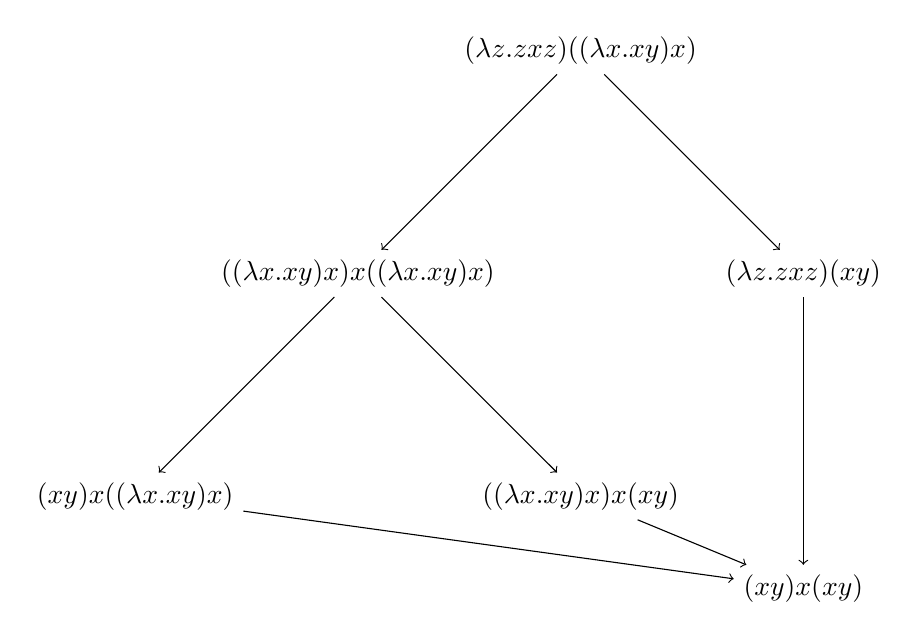
\begin{tikzpicture}[node distance =4 cm]
\node[](A){$(\lambda z. zxz) ((\lambda x. xy)x)$};
\node[](B)[below right of =A] {$(\lambda z. zxz)(xy)$};
\node[](C)[below of=B]{$(xy)x(xy)$};
\node[](D)[below left of = A]{$((\lambda x. xy)x) x ((\lambda x. xy)x)$};
\node[](E) [below left of = D]{$(xy)x((\lambda x. xy)x)$};
\node[](F) [below right of = D]{$((\lambda x. xy)x)x(xy)$};
\draw[->]
(A) edge (B)
(B) edge (C)
(A) edge (D)
(D) edge (E)
(D) edge (F)
(E) edge (C)
(F) edge (C);
\end{tikzpicture}

The $\beta$-normal form of $U$ is $(xy)x(xy)$.
\end{parts}
\end{solution}

% 1.8
\question 
Show that $(\lambda x. xx)y$ and $(\lambda xy. yx)xx$ are not $\beta$-convertible.
\begin{solution}
If they are $\beta$-convertible, then they must have the same $\beta$-normal form. However, the $\beta$-normal form of $(\lambda x. xx)y$ is $yy$ and the $\beta$-normal form of $(\lambda xy. yx)xx$ is $xx$.
\end{solution}

% 1.9
\question 
Consider the following terms 
\[K:=\lambda xy. x\]
\[S:=\lambda xyz. xz(yz)\]

\begin{solution}
Redexes are underlined for clarity. Application of a mult-argument function is shown as one step. 
\begin{parts}
\part
\[KPQ = \underline{(\lambda xy. x) P} \twoheadrightarrow_\beta P
\]
and 
\[\underline{SPQR}= \underline{(\lambda xyz. xz(yz)) PQR}\twoheadrightarrow_\beta PRQR
\]

\part
\[\underline{SKK} \twoheadrightarrow_\beta \lambda z. \underline{Kz(Kz)}\twoheadrightarrow_\beta \lambda z. z\]

\part
\begin{align*}
BUVW &= \underline{S(KS)KU}VW \\
&\twoheadrightarrow_\beta \underline{(KS)U}(KU)VW \\
&\twoheadrightarrow_\beta \underline{S(KU)VW }\\
&\twoheadrightarrow_\beta \underline{(KU)W}(VW) \\
&\twoheadrightarrow_\beta U(VW)
\end{align*}

\part
\[
\underline{SKKK} \twoheadrightarrow_\beta \underline{KK(KK)} \twoheadrightarrow_\beta K
\]
and 
\[
\underline{SSSK}K \twoheadrightarrow_\beta \underline{SK(SK)K} \twoheadrightarrow_\beta \underline{KK((SK)K)} \twoheadrightarrow_\beta K
\]
\end{parts}
\end{solution}
% 1.10 
\question Given the following
\[zero:=\lambda fx. x\]
\[one:=\lambda fx. f x\]
\[two:=\lambda fx. f (f x)\]
\[add:=\lambda mnfx. m f (n f x)\]
\[mult:=\lambda mnfx. m (n f) x\]
\begin{solution}
\begin{parts}
\part
\[\underline{\mathit{add} \mathit{one} \mathit{one}} \twoheadrightarrow_\beta \lambda fx. \underline{\mathit{one} f (\mathit{one} f x)} \twoheadrightarrow_\beta \lambda fx. f \underline{(\mathit{one} f x)} \twoheadrightarrow_\beta \lambda fx. f (f x) = \mathit{two} \]

\part
From (a) we know the $\beta$-normal form of $\mathit{add} \mathit{one} \mathit{one}$ is $\mathit{two}$. 
We also have
\[\underline{\mathit{mult} \mathit{one} \mathit{zero}} \twoheadrightarrow_\beta \lambda fx. \underline{\mathit{one} (\mathit{zero} f) x} \twoheadrightarrow_\beta \lambda fx. \underline{(\mathit{zero} f) x}  \twoheadrightarrow_\beta \lambda fx. x = zero\]
so the $\beta$-normal form of $\mathit{mult} \mathit{one} \mathit{zero}$ is $\mathit{zero}$, and $\mathit{two} \neq \mathit{zero}$
\end{parts}
\end{solution}
% 1.11
\question 

% 1.12
\question 

% 1.13
\question 

% 1.14
\question 

% 1.15
\question 

% 1.16
\question 

% 1.17
\question 

% 1.18
\question 

% 1.19
\question 

% 1.20
\question 

\end{questions}

\end{document}
